\chapter{Progettazione concettuale}
    \section{Class Diagram}

    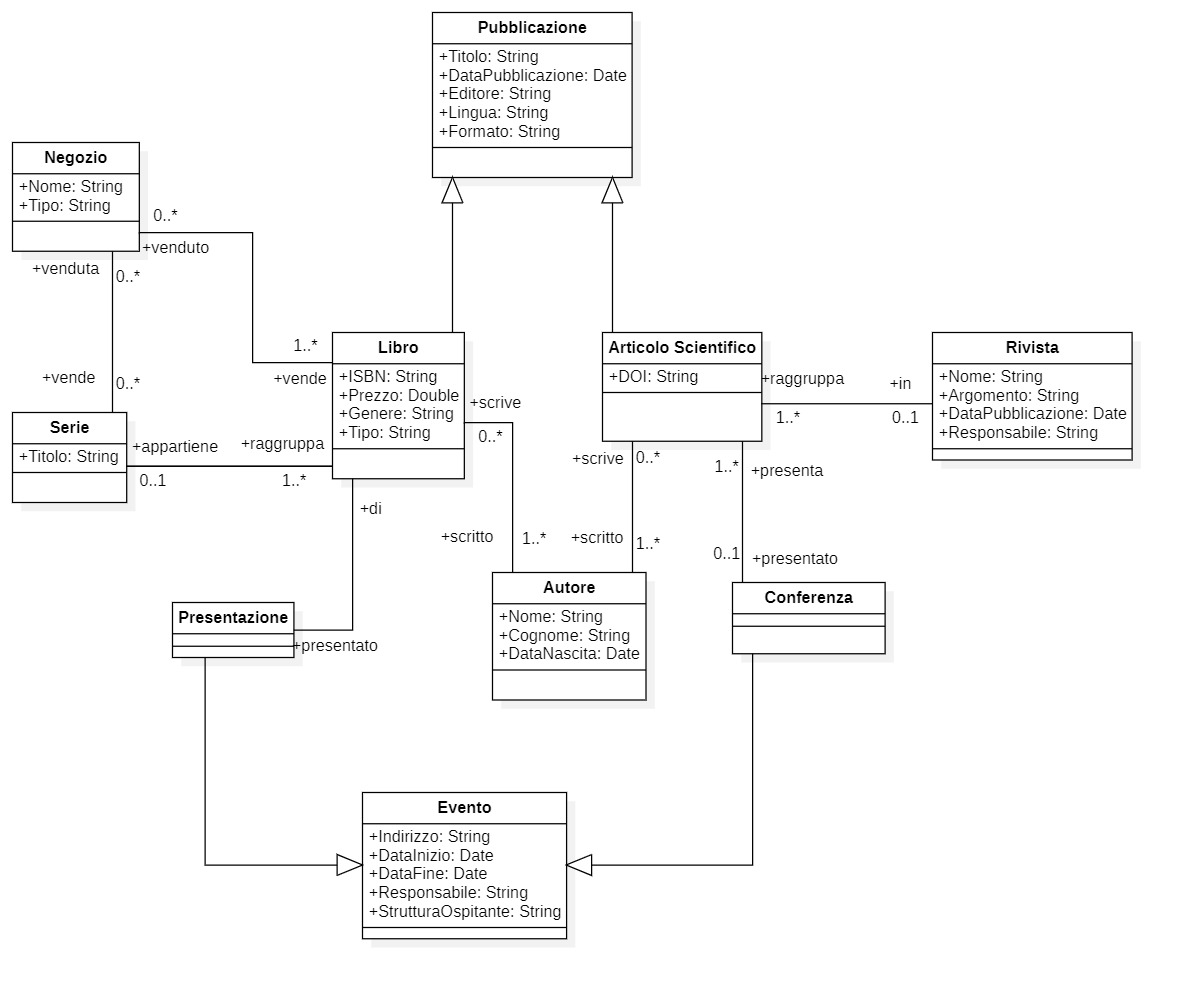
\includegraphics[scale=0.3]{Immagini/UML_v1_0.png}
        
    \section{Analisi della ristrutturazione del Class Diagram}
        In questa fase verranno effettueremo delle modifiche che renderanno il Class Diagram
        più adatto a una traduzione al modello logico \textcolor{red}{(magari scriviamo meglio sta parte)}
        \subsection{Analisi delle ridondanze}
        \textcolor{red}{(non saprei)}
        \subsection{Analisi degli identificativi}
        In questa fase andremo a scegliere uno o più attributi atti a identificare univocamente
        le varie entità presenti nello schema precedente, in particolare:
            \begin{enumerate}
            \item L'entità \textbf{Libro} presenta l'attributo ISBN che rappresenta una possibile chiave primaria,
                  tuttavia è stato scelto di aggiungere un attributo \textit{ID\_Libro} in modo tale da aumentare
                  la velocità di accesso agli indici.
            \item Per \textbf{Articolo scientifico} la situazione è analoga, è stato quindi aggiunto un attributo
                  \textit{ID\_Articolo}.
            \item Nel caso dell'entità \textbf{Rivista}, la quale presenta un attributo ISSN che è chiave candidata,
                  di inserire un ulteriore attributo \textit{ID\_Rivista}.
            \item Sarebbe possibile identificare un \textbf{Evento} tramite l
            \item L'entità \textbf{Conferenza} non possiede alcuna chiave candidata, si è ritenuto necessario quindi aggiungere
                  un attributo 
            \item \textbf{Presentazione}: 
            \item \textbf{Autore}: 
            \item \textbf{Negozio}:
            \item \textbf{Serie}: 
            \end{enumerate}
        \subsection{Rimozione degli attributi multipli}
            
        \subsection{Rimozione degli attributi composti}
            
        \subsection{Partizione/Accorpamento delle associazioni}
            
        \subsection{Rimozione delle gerarchie}
    
    \section{Class Diagram ristrutturato}
    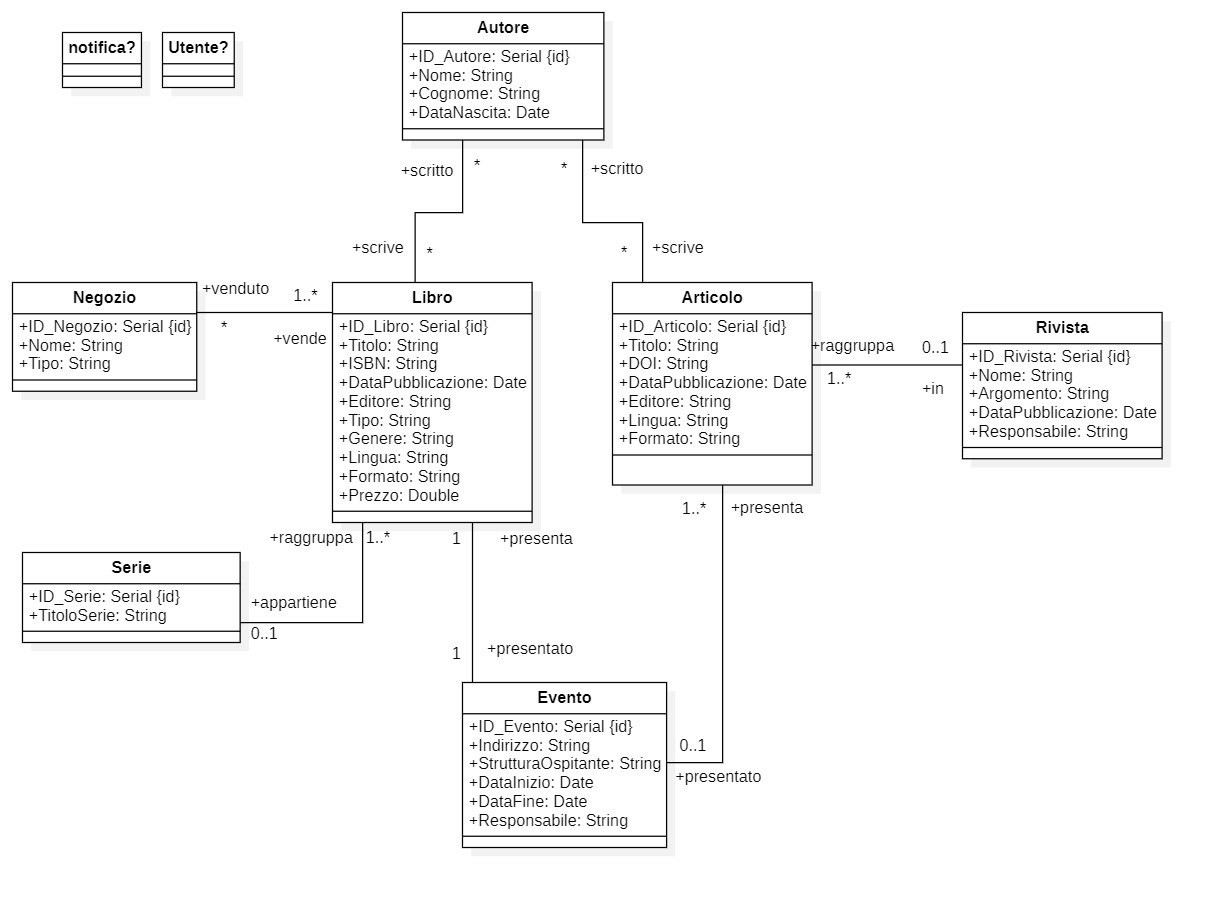
\includegraphics[scale=0.25]{Immagini/UMLris_v1_0.png}
        
    \section{Dizionario delle classi}
        
    \section{Dizionario delle associazioni}